\documentclass[a4paper]{jarticle}
\usepackage{sice-si}
\usepackage{amsmath} 
\usepackage[dvipdfmx]{graphicx}


\begin{document}
%
% タイトルと著者名
\title{STTによる会話中のキーワードごとのゲイン調整がタスクの遂行及びその際の身体運動に与える影響} % 和文タイトル
\name{○佐々部 岳人,天野 俊一(流通経済大学)} % 著者名
\etitle{Instruction for SICE SI Annual Conference Manuscript} % 英文タイトル
\ename{○Taro KEISOKU (SICE), and Hanako SEIGYO (SICE)}	%著者名(英)
%
% アブストラクト
\abst{
This manuscript describes a method for preparing a manuscript for the annual conference of the SICE SI division. 
}
% タイトルの出力
\maketitle
%
% 本文
\section{緒言}
本稿では SICE SI 部門講演会 SI の予稿原稿を作成するための説明を行います.
SIでは予稿原稿としてPDFファイル形式のファイルを電子投稿していただくことを原則とさせていただいております.
ただし,電子化やネットワーク接続が困難な場合には個別に対応させていただきますので,プログラム委員会までご相談ください(Webサイトからお問い合わせできます).
%
\section{ゲイン調整システム}
\subsection{システムの構成}
\begin{figure}[htbp]
    \begin{center}
    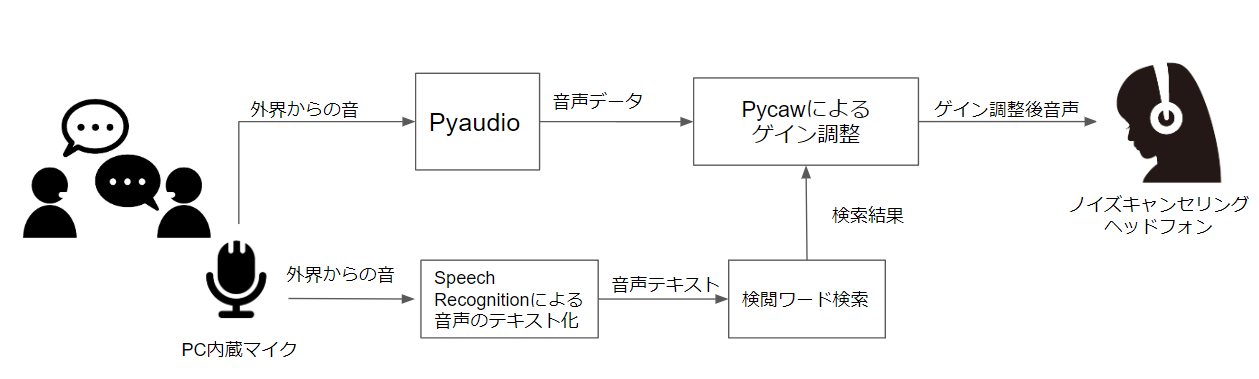
\includegraphics[width=80mm]{system.PNG}
    \caption{The device and the configuration.}
    \end{center}
    \end{figure}

こんなシステムの構成になっています.
\subsection{システムの効果}
    
システムを使っているときはこんな音の波形になっています.
\section{ゲイン調整システムの検証実験}
\subsection{実験概要}
\subsection{実験結果}
\subsection{ディスカッション}
%
%
%参考文献
\begin{thebibliography}{99}
\bibitem{SI}
	計測太郎,制御花子:
	``SICE SI予稿原稿の書き方(サンプル)'',  
   {\it 計測自動制御学会SI部門講演会SICE-SI予稿集}, 
    pp.0000--0000 (20??)
\end{thebibliography}
%
%
%
\end{document}

